\documentclass[tikz, border=0]{standalone}
\usepackage{tikz}
\begin{document}
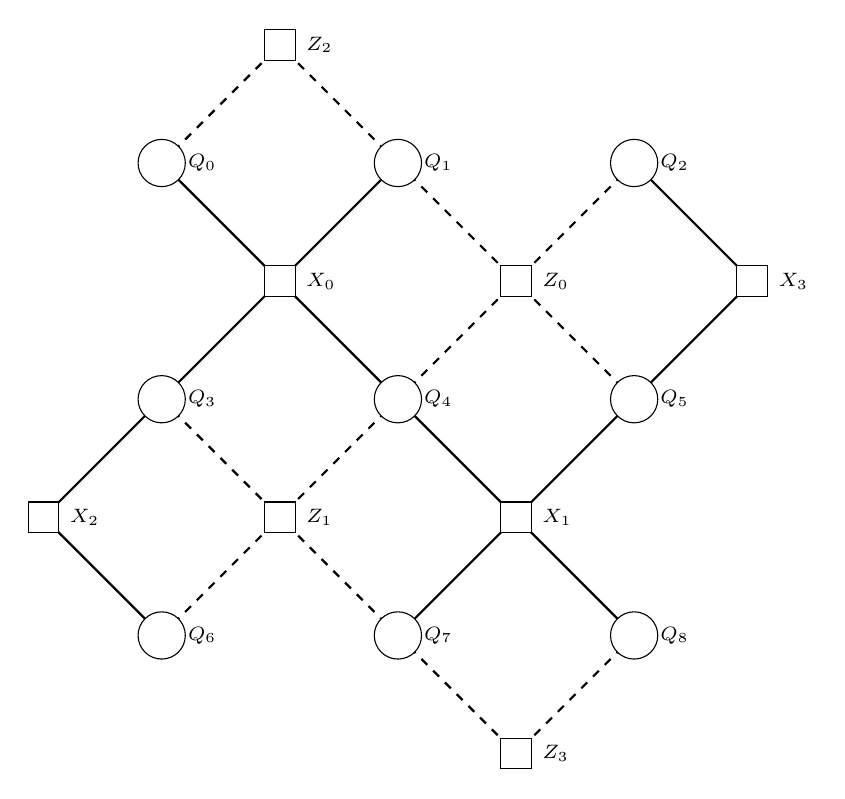
\begin{tikzpicture}
\draw[black,thick,solid] (0,6) -- (1.5,4.5);
\draw[black,thick,solid] (3,6) -- (1.5,4.5);
\draw[black,thick,solid] (0,3) -- (1.5,4.5);
\draw[black,thick,solid] (3,3) -- (1.5,4.5);
\draw[black,thick,solid] (3,3) -- (4.5,1.5);
\draw[black,thick,solid] (6,3) -- (4.5,1.5);
\draw[black,thick,solid] (3,0) -- (4.5,1.5);
\draw[black,thick,solid] (6,0) -- (4.5,1.5);
\draw[black,thick,solid] (0,3) -- (-1.5,1.5);
\draw[black,thick,solid] (0,0) -- (-1.5,1.5);
\draw[black,thick,solid] (6,6) -- (7.5,4.5);
\draw[black,thick,solid] (6,3) -- (7.5,4.5);
\draw[black,thick,dashed] (3,6) -- (4.5,4.5);
\draw[black,thick,dashed] (6,6) -- (4.5,4.5);
\draw[black,thick,dashed] (3,3) -- (4.5,4.5);
\draw[black,thick,dashed] (6,3) -- (4.5,4.5);
\draw[black,thick,dashed] (0,3) -- (1.5,1.5);
\draw[black,thick,dashed] (3,3) -- (1.5,1.5);
\draw[black,thick,dashed] (0,0) -- (1.5,1.5);
\draw[black,thick,dashed] (3,0) -- (1.5,1.5);
\draw[black,thick,dashed] (0,6) -- (1.5,7.5);
\draw[black,thick,dashed] (3,6) -- (1.5,7.5);
\draw[black,thick,dashed] (3,0) -- (4.5,-1.5);
\draw[black,thick,dashed] (6,0) -- (4.5,-1.5);
\filldraw[fill=white, draw=black] (0,6) circle (0.3) node at (0.21,6) [right] {$\scriptstyle Q_{0}$};
\filldraw[fill=white, draw=black] (3,6) circle (0.3) node at (3.21,6) [right] {$\scriptstyle Q_{1}$};
\filldraw[fill=white, draw=black] (6,6) circle (0.3) node at (6.21,6) [right] {$\scriptstyle Q_{2}$};
\filldraw[fill=white, draw=black] (0,3) circle (0.3) node at (0.21,3) [right] {$\scriptstyle Q_{3}$};
\filldraw[fill=white, draw=black] (3,3) circle (0.3) node at (3.21,3) [right] {$\scriptstyle Q_{4}$};
\filldraw[fill=white, draw=black] (6,3) circle (0.3) node at (6.21,3) [right] {$\scriptstyle Q_{5}$};
\filldraw[fill=white, draw=black] (0,0) circle (0.3) node at (0.21,0) [right] {$\scriptstyle Q_{6}$};
\filldraw[fill=white, draw=black] (3,0) circle (0.3) node at (3.21,0) [right] {$\scriptstyle Q_{7}$};
\filldraw[fill=white, draw=black] (6,0) circle (0.3) node at (6.21,0) [right] {$\scriptstyle Q_{8}$};
\filldraw[fill=white, draw=black] (1.305,4.305) rectangle (1.695,4.695) node at (1.7145000000000001,4.5) [right] {$\scriptstyle X_{0}$};
\filldraw[fill=white, draw=black] (4.305,1.305) rectangle (4.695,1.695) node at (4.7145,1.5) [right] {$\scriptstyle X_{1}$};
\filldraw[fill=white, draw=black] (-1.695,1.305) rectangle (-1.305,1.695) node at (-1.2854999999999999,1.5) [right] {$\scriptstyle X_{2}$};
\filldraw[fill=white, draw=black] (7.305,4.305) rectangle (7.695,4.695) node at (7.7145,4.5) [right] {$\scriptstyle X_{3}$};
\filldraw[fill=white, draw=black] (4.305,4.305) rectangle (4.695,4.695) node at (4.7145,4.5) [right] {$\scriptstyle Z_{0}$};
\filldraw[fill=white, draw=black] (1.305,1.305) rectangle (1.695,1.695) node at (1.7145000000000001,1.5) [right] {$\scriptstyle Z_{1}$};
\filldraw[fill=white, draw=black] (1.305,7.305) rectangle (1.695,7.695) node at (1.7145000000000001,7.5) [right] {$\scriptstyle Z_{2}$};
\filldraw[fill=white, draw=black] (4.305,-1.695) rectangle (4.695,-1.305) node at (4.7145,-1.5) [right] {$\scriptstyle Z_{3}$};
\end{tikzpicture}
\end{document}
